
To judge the degradation of algorithm predictions with decreasing information
quality (detailed in Section \ref{sec:inforeduc2}), a plot based on Figure
\ref{fig:detdemo} is presented for each energy window list (auto, short, and
long).  Figure \ref{fig:rxtr} shows the balanced accuracy of reactor type
classification for the previously described \textit{x}-axis, where a score of
$1$ is perfect prediction and a score of $0$ is random classification. The
error bars (which are not visible past the marker size on the plots) reflect a
99\% confidence interval.  The red baseline that indicates a minimum acceptable
performance is at 0.84 balanced accuracy, which is based on the lowest
performance of all three algorithms at 20\% training set error for the 29
nuclide mass training set in Figure \ref{fig:randrxtr}.  

\begin{figure}[!htb]
  \centering
  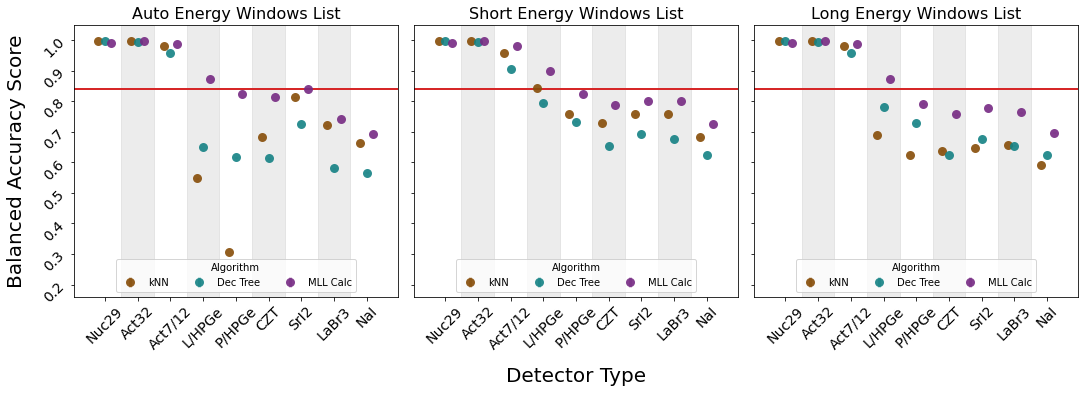
\includegraphics[width=\textwidth]{./chapters/exp2/detector_preds_wrt_enlist_BalAcc_rxtr.png}
  \caption[Prediction performance of reactor type classification with decreasing
           detector energy resolution]
          {Prediction performance of reactor type as measured by balanced 
           accuracy with respect to decreasing detector energy resolution 
           for three types of processed gamma spectra.}
  \label{fig:rxtr}
\end{figure}

The previous results in Figure \ref{fig:randrxtr} show the \textit{k}-nearest
neighbors line emerging with the lowest performance with decreasing
information, and it is interesting that this pattern did not emerge with the
detectors' performances in Figure \ref{fig:rxtr}.  Instead, for the auto and
short energy windows lists, the \textit{k}-nearest neighbors performance is
below \gls{MLL} calculations and above decision trees (except in the two unique
cases in the auto energy windows list).  For the lab-based and portable
\gls{HPGe}s, \textit{k}-nearest neighbors has the worst performance among all
three algorithms for the auto and long lists, and drastically so for the two
unique auto list cases of extremely poor performance.  In terms of the
baseline, there is only one instance of \textit{k}-nearest neighbors being
above it: the lab-based \gls{HPGe} with the short energy windows list. 

There are no detector-based training sets at all for which decision trees
performs above the baseline. For the last four detectors on the \textit{x}-axis
and all three energy windows lists, decision trees almost consistently performs
the worst. 

The \gls{MLL} calculations are the best performing algorithm on on three plots.
For the auto energy windows list, the lab-based \gls{HPGe} and \gls{SrI2}
detector-based training sets perform above the baseline. For the short and long
energy windows lists, only the lab-based \gls{HPGe} is above the baseline. 

Only the first three \textit{x}-axis categories exceed the baseline for all
three algorithms, which is expected for the various levels of full-knowledge
represented. The baseline may or may not be drawn at a reasonable level with
which to distinguish "acceptable" performance, but given its location, only the
lab-based \gls{HPGe} detector with \gls{MLL} calculations performs at an
acceptable level.

Next, the comparison of the gamma spectra processing will be discussed,
neglecting the baseline.  The short energy windows list performs the best
across the three methods used to process the gamma spectra. The auto energy
windows lists has one of the scintillator detectors (\gls{SrI2}) outperform the
baseline for \gls{MLL}, but the scikit-learn algorithms for the solid state
detectors perform erratically.  The variable behavior of the auto energy
windows list would require further study, but the fact that the \gls{SrI2}
detector outperforms all of the solid state detectors speaks to how an
automatic peak search should not be discarded as a method.  The auto energy
windows list set of points for \gls{SrI2} outperforms even the portable
\gls{HPGe} on the short energy windows list.  The slightly worse outcomes for
the long energy windows list are to be expected from the algorithms having to
deal with a lot of non-useable features, especially for the last four
detectors, since their spectra will not contain measurable peaks from many of
the gamma energies in that list. 

\begin{figure}[!htbp]
  \centering
  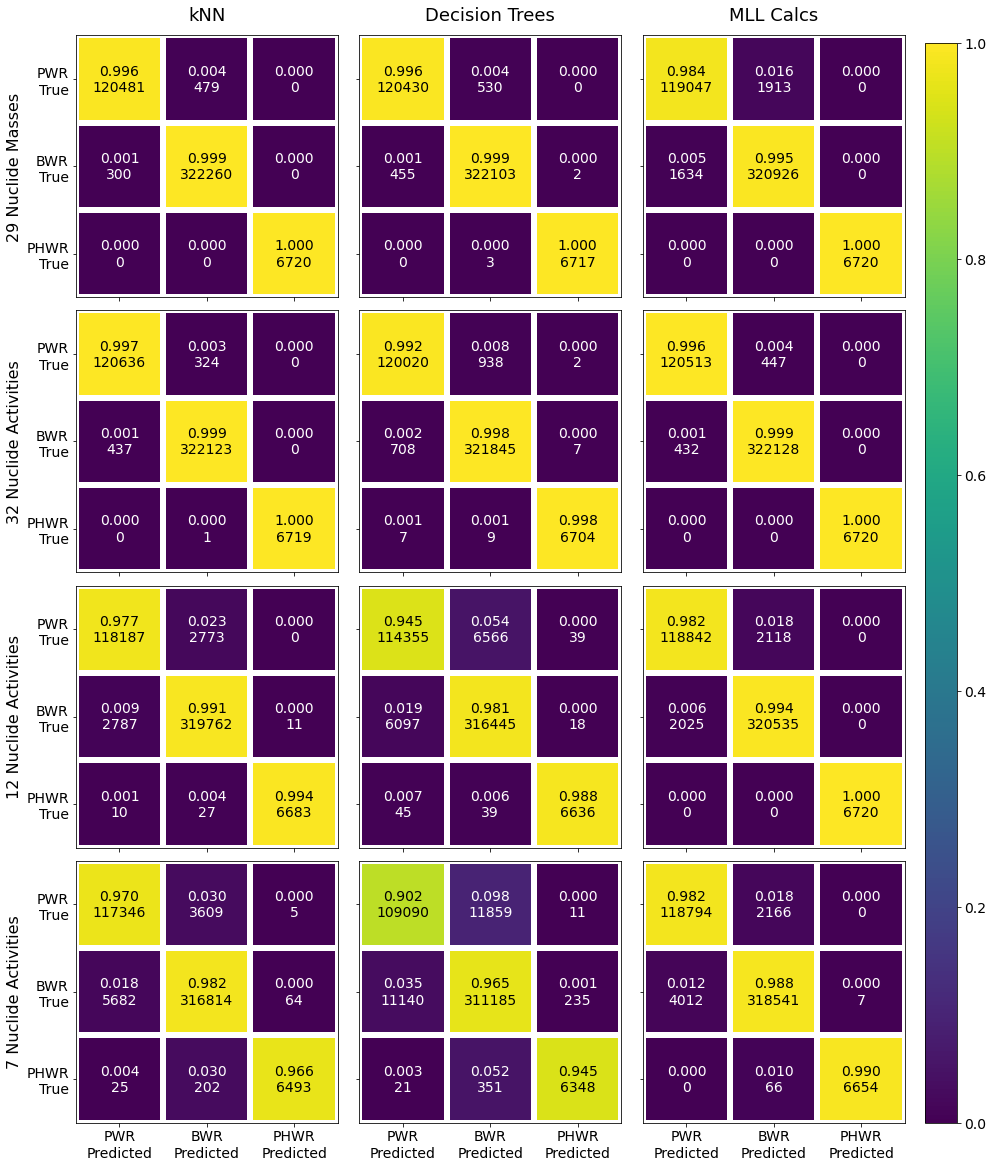
\includegraphics[width=\textwidth]{./chapters/exp2/confusion_matrix_nucs_acts.png}
  \caption[Confusion matrices of reactor type classification for non-detector 
           training sets]
          {Confusion matrices of reactor type prediction for each algorithm 
           for different training sets (all at a 1\% error level): 29 nuclide 
           masses, 32 nuclide activities, 12 nuclide activities, and 7 nuclide 
           activities.}
  \label{fig:cm_nucs_acts}
\end{figure}

As in Section \ref{sec:randerr}, the reactor type classification performance
discussion would not be complete without the added detail that confusion
matrices supply (see Sections \ref{sec:testerr} and \ref{sec:randerrA} for an
introduction to confusion matrices).  First, the four "full knowledge" training
sets are presented in Figure \ref{fig:cm_nucs_acts}.  Note that the color bar
extends from -0.1 to 0.1, which is a very small range.  The results in all four
panels are all quite accurate, so a small color bar range is necessary to make
a visual distinction of performance relative to the other full knowledge cases.
The 29 nuclide mass training set (top panel) is repeated from the 1\% training
set error case in Figure \ref{fig:cm_nuc29}.  For the 32 nuclide activity
training set (second panel), the numbers are approximately the same, but
interestingly, they improve slightly for \textit{k}-nearest neighbors and
\gls{MLL} calculations.  A visible increase in misclassification is clear with
the 12 and 7 nuclide activity training sets, especially for decision trees. The
starkest increase in misclassification is with \gls{PWR}s being classified as
\gls{BWR}s. This increases from about 5\% to about 10\% from the 12 nuclides
set to the 7 nuclides set. For the 7 nuclides set decision trees
classification, the misclassification of \gls{PHWR}s as \gls{BWR}s reaches
about 5\%. By contrast, the same misclassification is 3\% for
\textit{k}-nearest neighbors and 1\% for \gls{MLL} calculations. 

\begin{figure}[!htbp]
  \centering
  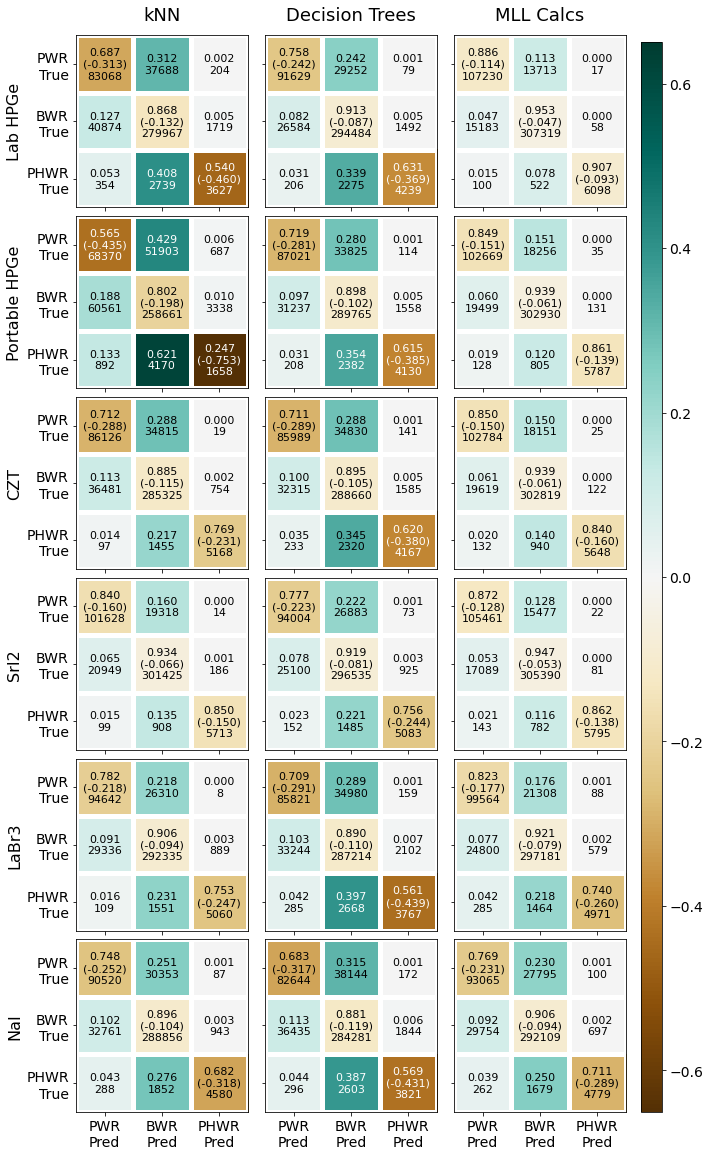
\includegraphics[width=0.83\textwidth]{./chapters/exp2/confusion_matrix_6dets_auto.png}
  \caption[Confusion matrices for auto energy window list training sets.]
          {Confusion matrices for auto energy window list training sets.}
  \label{fig:cm_auto}
\end{figure}

\begin{figure}[!htbp]
  \centering
  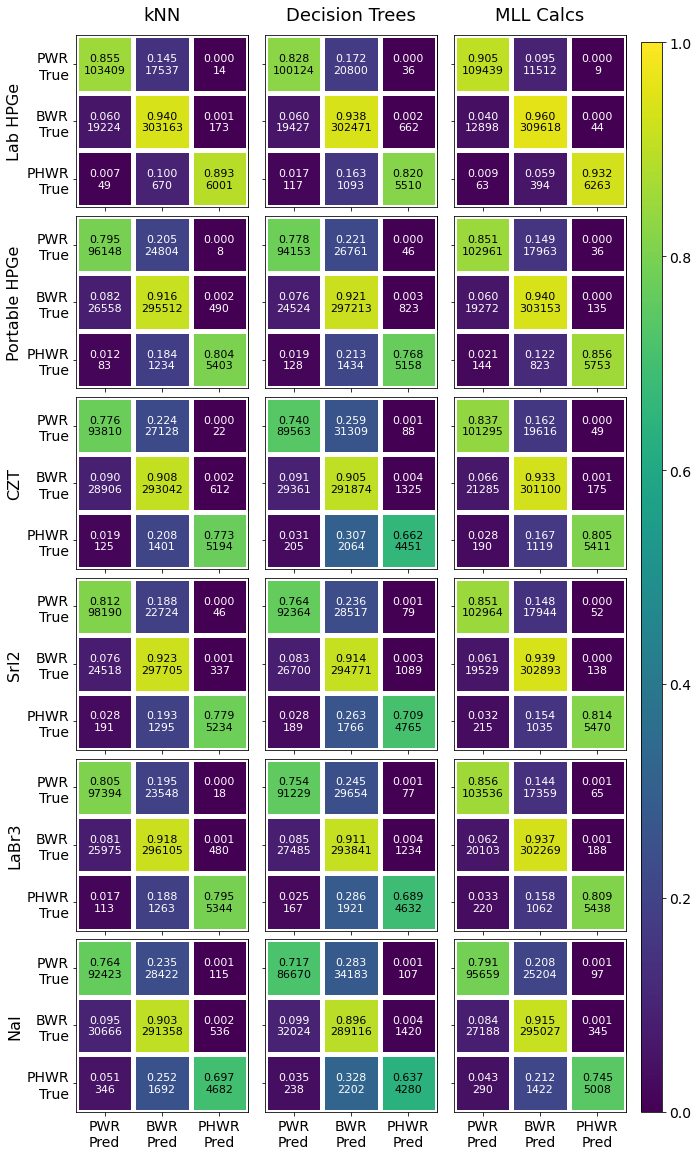
\includegraphics[width=0.83\textwidth]{./chapters/exp2/confusion_matrix_6dets_short.png}
  \caption[Confusion matrices for short energy window list training sets.]
          {Confusion matrices for short energy window list training sets.}
  \label{fig:cm_short}
\end{figure}

\begin{figure}[!htbp]
  \centering
  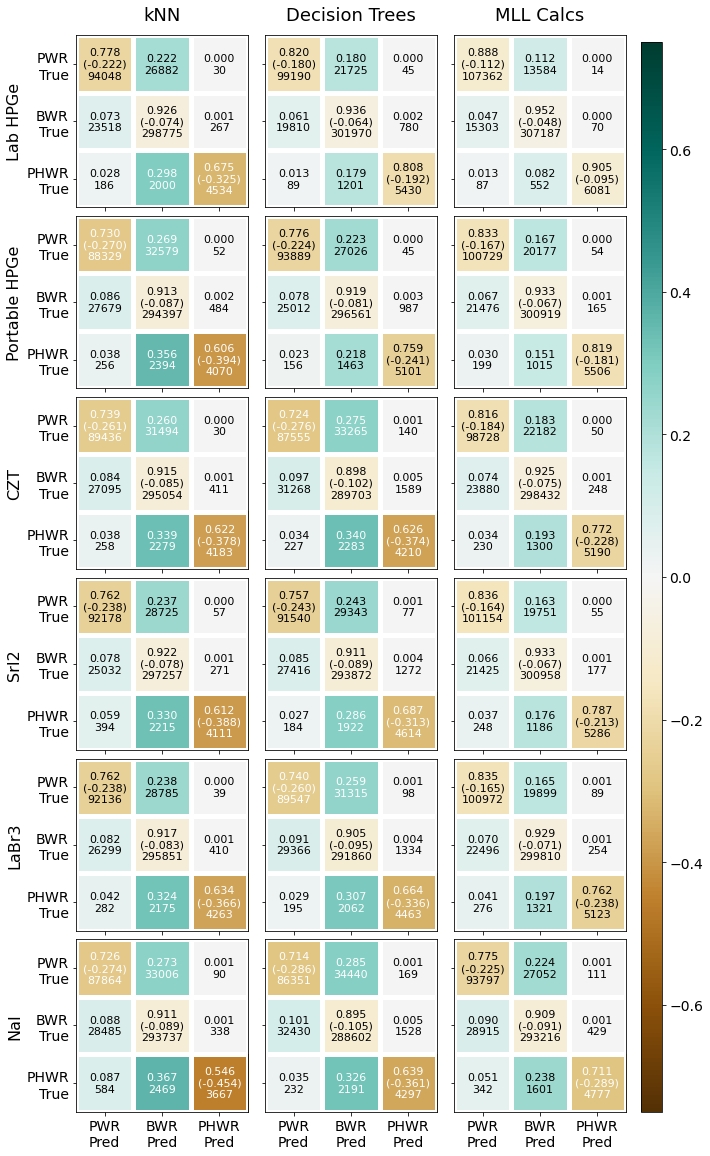
\includegraphics[width=0.83\textwidth]{./chapters/exp2/confusion_matrix_6dets_long.png}
  \caption[Confusion matrices for long energy window list training sets.]
          {Confusion matrices for long energy window list training sets.}
  \label{fig:cm_long}
\end{figure}

Next, Figures \ref{fig:cm_auto}, \ref{fig:cm_short}, and \ref{fig:cm_long} show
the confusion matrices for all six detectors (in the same order top-to-bottom
as the \textit{x}-axis in Figure \ref{fig:rxtr}) for the auto, short, and long
energy windows list training sets, respectively. For these figures, the color
bar range is much wider (-0.65 to 0.65) than with the more accurate results in
Figure \ref{fig:cm_nucs_acts}. 

In Figure \ref{fig:cm_auto}, the two poorly performing \textit{k}-nearest
neighbors \gls{HPGe} cases are the most noticeable confusion matrices visually.
The \textit{k}-nearest neighbors performances for the two \gls{HPGe}s were
notably poor in the plot, and the confusion matrices for these two cases
explains why: not only are 40.8\% and 62.1\% of \gls{PHWR}s being misclassified
as \gls{BWR}s for the lab-based and portable \gls{HPGe}s, respectively, 31.2\%
and 42.9\% of the \gls{PWR}s are misclassified as \gls{BWR}s for the same two
detectors, respectively.

By contrast, the anomalous high performance of the \gls{SrI2} detector training
set, for all three algorithms, can be seen in its panel that is paler in over
color than its surroundings.  The confusion matrix (in the fourth panel) for
those data points show no more than 16\% of \gls{BWR}-misclassified \gls{PWR}s
and \gls{PHWR}s for \textit{k}-nearest neighbors, no more than 23\% for
decision trees and no more than 13\% for \gls{MLL} calculations. 

Aside from the two poorly performing \textit{k}-nearest neighbors cases, the
decision trees column has the boldest colors/poorest performance.  The lowest
\gls{BWR} misclassification value is 22\%.  Additionally, it can be visually
perceived at a glance that the \gls{MLL} column has better performance than the
other two algorithms. This is expected from the higher balanced accuracy scores
in Figure \ref{fig:rxtr}.  Throughout all six panels, the highest
misclassification value is 25\%.

Next, Figure \ref{fig:cm_short} is on the following page, providing more detail
about the reactor type classification than is seen in the middle plot in Figure
\ref{fig:rxtr}.  The better classification performance across all algorithms
can be seen instantly, since the color bar spans the same range as with Figure
\ref{fig:cm_auto}. Again, the relatively poor performance of decision trees can
be seen with the bolder colors compared to the two other algorithms. For
decision trees, the misclassification of \gls{PHWR}s as \gls{BWR}s reaches
32.8\%, whereas those values are 25.2\% for \textit{k}-nearest neighbors and
21.2\$ for \gls{MLL} calculations.

Last, Figure \ref{fig:cm_long} provides more classification detail on the third
plot in Figure \ref{fig:rxtr}. The \gls{MLL} performance takes a similar shape
at a slightly lower balanced accuracy score compared to the short auto energy
windows list, seen in Figure \ref{fig:rxtr} and in the comparison of Figures
\ref{fig:cm_short} and \ref{fig:cm_long}. What makes the long energy windows
list results unique is that \textit{k}-nearest neighbors and decision trees
have very close balanced accuracy scores for the bottom four detectors. By
looking at their confusion matrices, one can see that the misclassification
patterns are also similar. The first two detectors, both of the \gls{HPGe}s,
have notably lower classification performance for \textit{k}-nearest neighbors,
however. This may or may not be related to the reason the two training sets
from these detectors perform significantly worse for the auto energy windows
list. 

The two extreme \textit{k}-nearest neighbors cases for the two \gls{HPGe}s is a
behavior that will repeat for not-yet-discussed prediction parameters.  The
most likely explanation is that the automatic peak search step (as opposed to
predefining the selection of peaks based on expected gamma energy photopeaks)
finds peaks that are adding noise and not information to the energy windows
lists.  Since these algorithms all suffer from high variance, it is possible
that this peak search approach is causing these two detectors (which have a
high energy resolution) to succumb to the additional noise. This should be
contrasted with the case of the \gls{SrI2} detector, where it is one of the
only detector-based training sets to exceed the baseline defined level.

Overall, the sets of confusion matrices presented in Figures
\ref{fig:cm_nucs_acts}-\ref{fig:cm_long} show various degrees of the same
misclassification pattern. With less information, more \gls{PWR}s and
\gls{PHWR}s get classified as \gls{BWR}s. Since about 72\% of the training set
is an entry on \gls{BWR}, this pattern is expected.

